% Thank you for the invitation and the kind introduction.
% Good afternoon and welcome! I'll give a glimpse into symplectic geometry and holomorphic curves. This is a broad field, so many things I cannot tell you - but let me show you three questions which I *will* talk about.

\section{introduction}
\begin{frame}
  \frametitle{Three motivating questions}
  % The first question is about the so-called filling problem: when is a manifold the boundary of a compact manifold one dimension higher?
  \begin{block}{Question 1: symplectic fillings}
    When is a smooth manifold the boundary of a compact manifold?
  \end{block}
  % Secondly, if you have an elliptic partial differential equation, what can we expect its solution space to look like?
  \begin{block}{Question 2: moduli spaces}
    What does the solution space to an elliptic PDE look like?
  \end{block}
  % Thirdly: what can we say about periodic orbits of a mechanical system?
  \begin{block}{Question 3: dynamical systems}
    What can we say about periodic orbits of a mechanical system\\(e.g. double pendulum, the solar system)?
  \end{block}
  % There are more questions we could put here. For instance, Shah Faisal will talk about symplectic embedding problems tomorrow.
\end{frame}

% I hope there's an interesting question for you. Let's dive in and set the stage for our first hero, symplectic manifolds.
% "manifold", I hear you ask. Let me start by quickly explaining that.
\begin{frame}
  \frametitle{Smooth manifolds}
  % Imagine you're an ant crawling over the surface of the earth. You can move in two independent directions: forwards or backwards, and left or right. Let's pretend you're *really* small, so you don't notice that earth is uneven: to you, whereever you are, near you the surface of the earth looks like (part of) a disc.
  \makebox[\textwidth]{\framebox[5cm]{
    \rule{0pt}{5cm}
  }}
  \makebox[\textwidth]{picture of an ant crawling across the earth}
  % TODO: picture of the ant; perhaps two different pictures
  % In other words: earth' surface is an object which, locally looks, to an ant, like a part of a disk.
  earth is a manifold: locally looks like part of a disk
\end{frame}

\begin{frame}
  \frametitle{Smooth manifolds}
  % Let's generalise that to higher dimensions: an n-dimensional manifold M is a topological space which locally looks like R^n. We also call a two-dimensional manifold a surface.
  \begin{itemize}
    \item manifold: \shrink{second countable Hausdorff} topological space $M$ locally homeomorphic to $\R^n$

    % every point has an open nbhd homeomorphic to R^n (a coordinate chart); these charts overlap and transition functions are homeo
    \item every $p\in M$ has a coordinate chart:\\$p\in U\subset M$ open, homeomorphism $\phi\colon V\to U$ for $V\subset \R^n$
    % these charts form an open cover of $M$; the open cover of all charts is part of the datum of the manifold
    % whenever two charts overlap: there is a resulting coordinate transformation (which is a homeomorphism)
    % There are two technical details which I will not go into: we assume our space to be Hausdorff and second countable. Don't worry if you don't know what this means; basically all examples I would encounter in nature are these.

    % I'm a differential geometer, so all my manifolds today are smooth. This just means all transition maps between different charts are smooth.
    % One can have different smooth structures on the same topological manifold; we always talk about a manifold with a chosen smooth structure.
    % This is a restriction, but often not a big one. "Many" topological manifolds have a smooth structure; there are notably some manifolds which are not. (This is part of what Simon Donaldson got his fields medal for in 1986.)
    \item smooth manifold: all coordinate transformations from overlapping charts are smooth
  \end{itemize}
  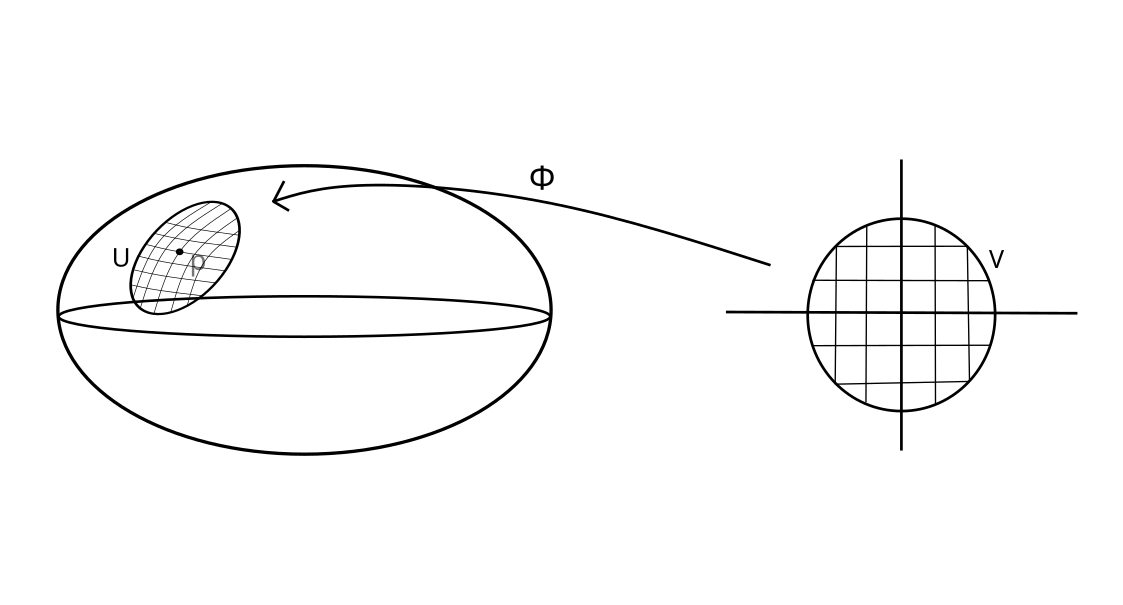
\includegraphics[width=8cm]{images/surface_with_chart.png}
\end{frame}

\begin{frame}
  \frametitle{(Non-)Examples of smooth manifolds}
  % Let's look at some examples of manifolds.
  \begin{itemize}
  % In general, taking the (disjoint) union of two n-manifolds yields another n-manifold - so we can focus on connected spaces.
  % A zero-dimensional manifold is a point (or several disconnected points) -- not interesting.
  % In dimension 1, we can have a line, but also a circle (and unions of those).
  \item $n=1$: $\R$, $\sphere{1}$ % TODO: add pictures!
  \framebox[1cm]{line}\framebox[1cm]{circle}
  %\includegraphics[width=1cm]{images/line.png}
  %\includegraphics[width=1cm]{images/circle.png}
  % in dimension two, things get more interesting: the earth's surface is such an example.
  % topologically, it's homeomorphic to a sphere (or perhaps your favourite potato); we can also have a doughnut (or coffee cup) - but we could also take g tori and squish them together in a line (as drawn here). You'd call that a closed genus g surface.
  \item $n=2$: $\R^2$, $\sphere{2}$, $\T^2$, $\Sigma_g$ for $g\geq 1$\\
  \raisebox{4pt}{\mbox{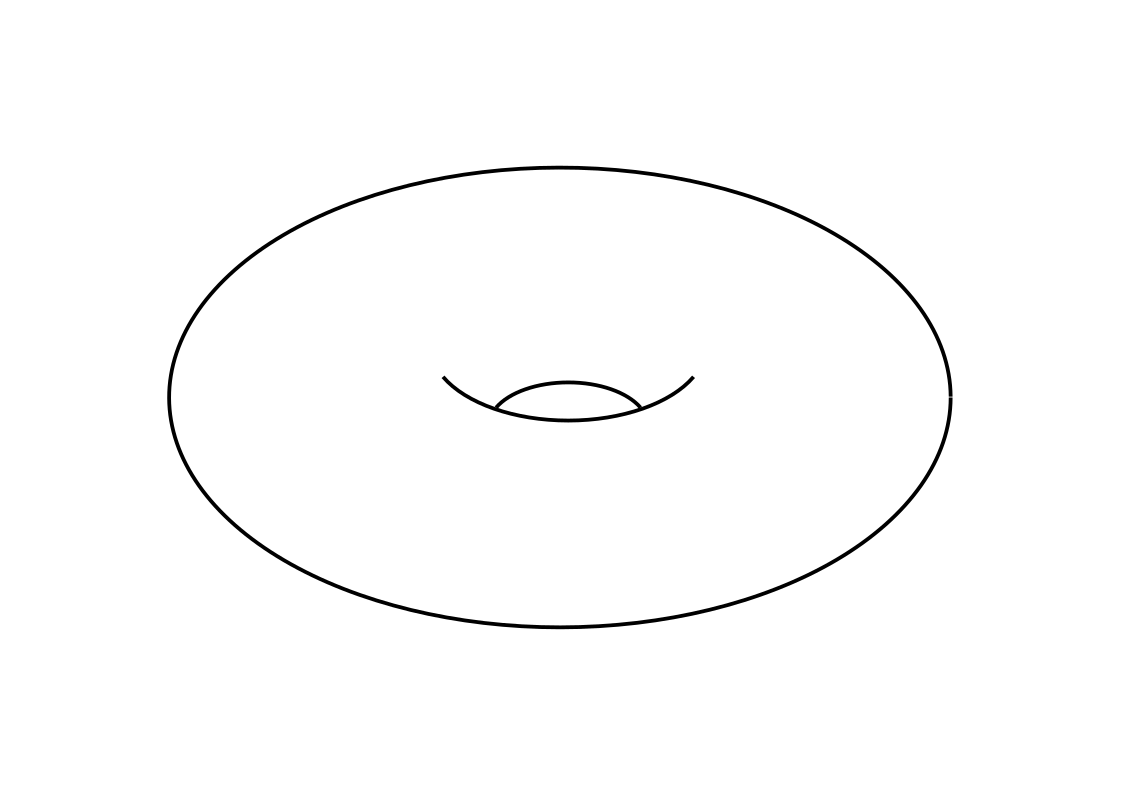
\includegraphics[width=1cm]{images/torus.png}}}
  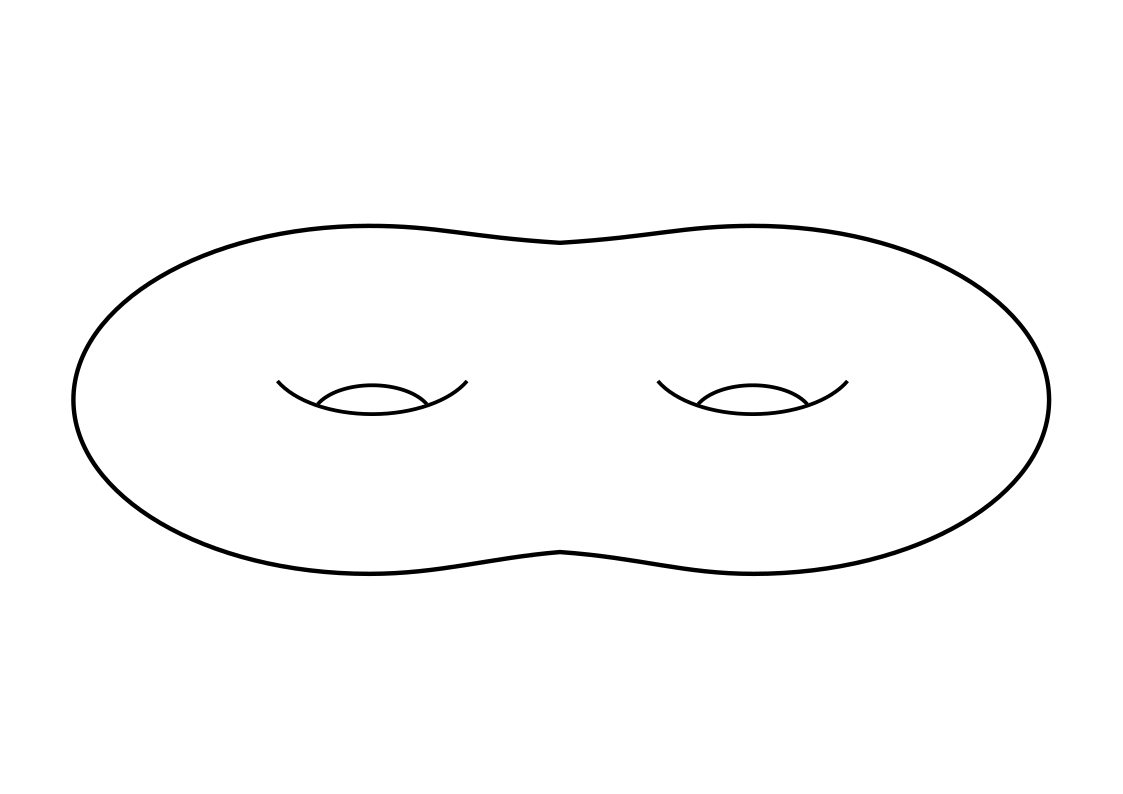
\includegraphics[width=1.5cm]{images/surface_genus_2.png}
  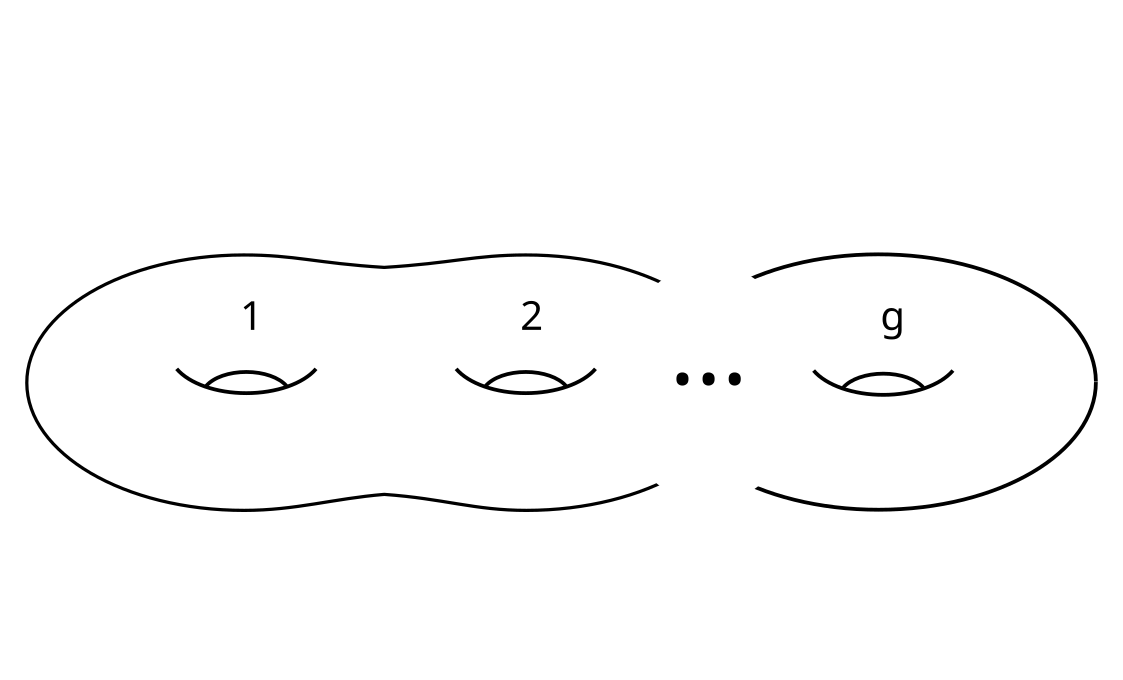
\includegraphics[width=2cm]{images/surface_genus_g.png}
  % in three dimensions, you have the three-sphere and 3-torus, but also real projective space; there's a whole zoo of other 3-manifolds
  % you don't have a nice list of manifolds as in dimension two, but you still have an explicit classification
  \item $n=3$: $\R^3$, $\sphere{3}$, $\T^3$, $\RP{3}$
  % from dimension four onwards, things get much wilder. a classification is provably impossible; even e.g. simply connected ones are HARD
  \item $n=4$: $R^4$, $\sphere{4}$, $\T^4$, $\CP{2}$, $\CP{2}\#\overline{\CP{2}}$
  % FIXME: compare with Thomas' talk and insert more examples
  \end{itemize}
  % And some things which are not a manifold: the letter X is not a 1-dimensional manifold (at the crossing, it's not homeomorphic to a line segment)
\end{frame}

% Next, what is a symplectic manifold? To describe these, let's focus on dimension two first.
% How do you measure area in two dimensions? Given a small patch of a (smooth) surface, how shall we measure or define its area?
\begin{frame}
  \frametitle{How to measure area on a 2-manifold?}
  \begin{itemize}
  % For a subset of R^n, we obtain the area by integrating its characteristic function (w.r.t. a suitable measure).
  % If our patch is sufficiently small, we map it to R^2 via a chart and determine the area there: this amounts to integrating over a density function. Globally, we need to choose density functions in each chart in a compatible way: this amounts to a differential 2-form.
  \item locally: integrate density function
  \item globally: use a differential 2-form
  % To make this precise, we consider the *tangent space* at a point. Imagine the manifold placed inside some R^n (the Whitney embedding theorem tell us we can always do this). Geometrically, the tangent space at a point is the space of all vectors at this point which are tangent to a manifold. I'll skip a formal definition.
  % This is a real vector space, of the same dimension as the manifold. Moreover, a local chart induces a basis of the tangent space.
  \item each $p\in M$ has \highlight{tangent space} $T_pM$, $2$-dimensional
  % Now, a differential two-form locally specifies a density function for each local chart. Formally, it's a family of skew-symmetric bilinear maps on each tangent space, varying smoothly along the base point.
  \item $2$-form $\omega = \{\omega_p\colon T_pM\times T_pM\to \R\}_{p\in M}$\\ $\omega_p$ anti-symmetric bilinear, smoothly varying with $p$
  % We call a 2-form an area form if each bilinear map is non-degenerate.
  \item \highlight{area form}: each $\omega_p$ is non-degenerate
  % A two-dimensional symplectic manifold is precisely a smooth surface with a choice of area form.
  \item \highlight{symplectic $2$-manifold}: $M$ plus choice of area form
\end{itemize}
\end{frame}

\begin{frame}
  \frametitle{Symplectic manifolds}
  % In general, a symplectic structure on a smooth manifold is a choice of a non-degenerate closed 2-form. Non-degeneracy means each bilinear form is non-degenerate; closedness means its exterior derivative vanishes.
  \begin{definition}
    A symplectic manifold $(M,\omega)$ is a smooth manifold $M$ together with a closed non-degenerate $2$-form $\omega$.
  \end{definition}
  % For example, every orientable surface is a symplectic manifold: take any area form (which is automatically closed by dimension reasons).
  % Probably that definition wasn't very illuminating. Let's give a more geometric explanation. A symplectic structure assigns signed area of all (sufficiently local) closed curves.
  \begin{itemize}
    \item equivalently: atlas of charts $(x_1,y_1,\dots,x_n,y_n)$\\
    in which $\omega$ looks like $\omega_0=\sum_{i=1}^n dx^i\wedge dy^i$
    \item geometrically: symp.\ structure = signed area of closed curves
    % Consider an embedded closed curve in R²: it bounds a closed disc (by the Jordan curve theorem). Consider the area of this disc.
    \item for $\gamma$ embedded closed curve in $\R^2$ $\to$ $A(\gamma)$ signed area of enclosed disc
    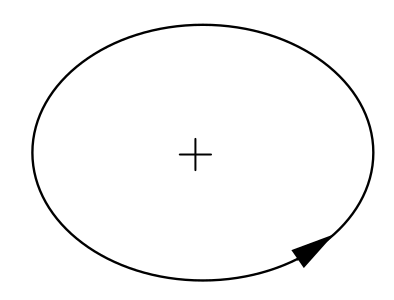
\includegraphics[width=2cm]{images/curve_orientation1.png}\pause
    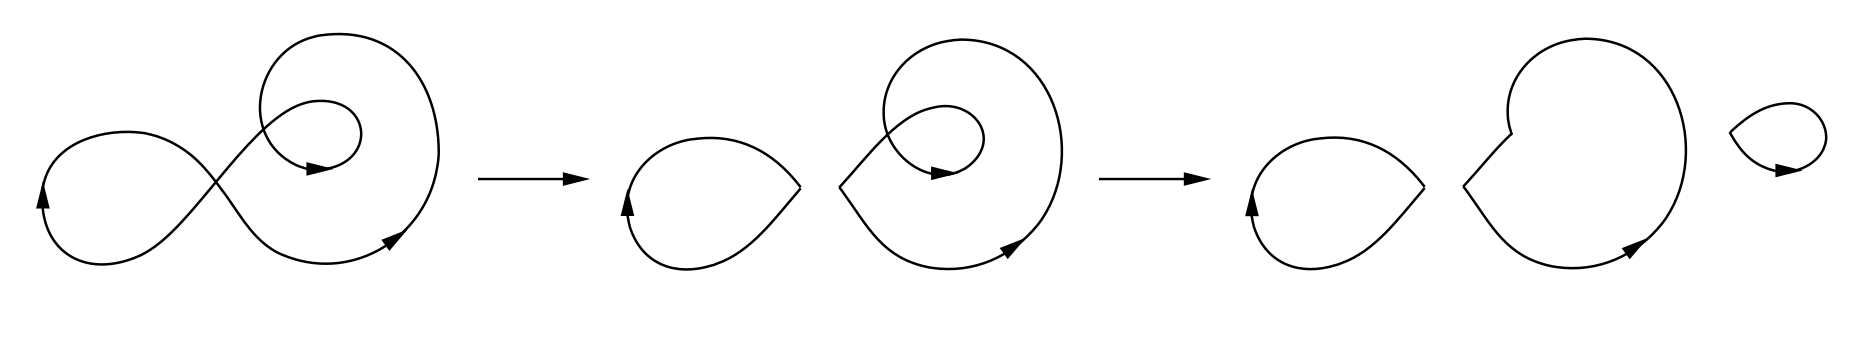
\includegraphics[width=7cm]{images/splitting_nonembedded_curve.png}
    \item $\gamma$ any oriented closed \shrink{piece-wise smooth} curve:\\ decompose into closed embedded pieces
  \end{itemize}
\end{frame}

\begin{frame}
  \frametitle{Symplectic manifolds (geometric definition)}
  \begin{itemize}
    \item \highlight{standard symplectic structure} on $\R^{2n}$:\\
    map $\gamma\to A(\gamma)=A(\gamma_1)+\dots+A(\gamma_n)$,\\
    where $\gamma=(\gamma_1,\dots,\gamma_n)$ any closed oriented curve
    % Given a smooth manifold, choose an atlas: for any closed curve contained in a coordinate chart, we can determine its signed area.
    % A symplectic structure is a compatible way of making such choices.
    % In other words, it's an atlas whose transition functions preserve signed area.
    \item symplectic structure on $M$ is an atlas whose transition functions preserve signed area
    % why are these definitions the same? if \gamma bounds the disc D, Stokes shows A(\gamma)=\int_D \omega_std. Darboux' shows a symplectic structure is an atlas whose transition functions are symplectomorphisms.
    \item equivalence: Darboux' theorem and short computation
  \end{itemize}
\end{frame}
